\cleardoublepage
\chapter{Introduksjon}
\label{chap:intro}

\section{Prosjektgruppen}
%-----------Sørge for å dele opp de 4 gruppemedlemmene med litt luft.--------------%
Prosjektgruppen er sammensatt av fire studenter ved IT-avdelingen ved Høgskolen i Østfold, tre fra Digitale Medier og Design og én student fra Informatikk - Design og utvikling av IT-systemer.

Ingrid Elise Dahl studerer Informatikk - Design og utvikling av IT-systemer, bor i Halden og er fra Trondheim. Ingrids faglige interesser innebærer frontend-utvikling, design, datasikkerhet, databasesystemer og applikasjonsutvikling.

Markus Arnø Madsen studerer Digitale medier og Design, bor i Fredrikstad og er fra Trondheim. Markus sin faglige interesse innebærer design, prosjektledelse, interaksjons design, brukerorientert design, markedsføring og prosjekt/produkt utvikling.

Anders Walle Pettersen studerer Digitale medier og Design, bor i Fredrikstad. Anders sin faglige interesse innebærer design, interaksjons design, spillutvikling, grafisk design og brukerorientert design.

Stefan Larsen studerer Digitale medier og Design, og bor i Halden. 3D og Grafisk design, samt Webutvikling har vært noen av de mest interessante veiene å utforske gjennom studietiden på HIOF. 


\section{Oppdragsgiver}
Prosjektgruppens oppdragsgiver er Tommy Payne på vegne av Høgskolen i Østfold (omtalt som HIØ videre i dokumentet). HIØ har 7700 studenter og 620 ansatte fordelt på to campus i Halden og Fredrikstad\footnote{https://www.hiof.no/om/}. Det er fem fagavdelinger, ett akademi og ett senter ved HIØ\footnote{https://www.hiof.no/om/organisasjon/fagavdelinger/}.

Tommy Payne jobber som Seniorkonsulent i Studieenheten ved HIØ og inngår i team for Studieutredning og kvalitetssikring med ansvar for det helhetlige læringsmiljøet ved campus Halden og campus Fredrikstad. Arbeidet hans går ut på å sikre og videreutvikle det digitale, fysiske, organisatoriske og psykososiale læringsmiljøet ved høgskolen. \footnote{https://www.hiof.no/om/organisasjon/administrasjonen/organisasjons-og-tjenesteutvikling/studenttjenester/personer/tekn-adm-ansatte/tommypa/}

\section{Oppdraget}
Løsningen som gruppen har kommet fram til i samråd med oppdragsgiver er en prototype av en nettbasert tjeneste for studenter der de kan finne organisasjoner, lag og foreninger i sitt nærområde. Prototypen skal bestå av et sett med klikkbare skisser laget i verktøyet Adobe XD. Prosjektet baserer seg på at gruppen skal levere denne prototypen sammen med hoveddokumentet til oppdragsgiver, hvor disse kan fungere som et utgangspunkt med instruksjoner for å muliggjøre utviklingen av prototypen til ferdig stand på et senere tidspunkt. En av løsningene som skal skisseres i prototypen er innhenting av informasjon om organisasjoner, lag og foreninger fra Brønnøysundregistrene \footnote{https://www.brreg.no/}, i tillegg til en løsning som oppfordrer organisasjoner til å registrere informasjon om seg selv.

Oppdragsgiver Tommy Payne jobber med læringsmiljø og studentenes trivsel og helse ved HIØ. Å utvikle en løsning som kan bidra til at studenter blir mer aktive, deltar mer sosialt og engasjerer seg i lokalmiljøet vil være av interesse for både studentene, Tommy Payne, HIØ som institusjon og nærmiljøet rundt Høgskolen.

\paragraph{Tillegg og endringer fra prosjektbeskrivelsen}
Notater:
Prototype istedenfor ferdig tjeneste.
Ingen webcrawler eller automatisk henting av informasjon.
Mulighet for kontakt mellom brukere - sosialt aspekt.
System som foreslår aktiviteter til brukeren.

\subsection{Problemstilling}
Studenter ved HIØ har pr. i dag ikke tilfredsstillende verktøy for å finne oversikt over fritidsaktiviteter og ta kontakt med organisasjoner som arrangerer disse. Hvordan kan man designe et verktøy som legger til rette for at studenter enklere kan delta på fritidsaktiviteter og ta kontakt med organisasjoner, lag og foreninger i sitt nærområde? Hvordan kan tjenesten utformes på en måte som gjør det interessant og attraktivt for studenter å gjøre dette? Hvordan kan denne tjenesten synliggjøres for både studenter og organisasjoner, lag og foreninger med den hensikt at den skal bli brukt av flest mulig i målgruppen?

\subsection{Utvikling av hypoteser}
\label{section:hypoteser}
Prosjektgruppen utviklet fire hypoteser som i løpet av prosjektet ble utforsket gjennom brukerintervjuer -og undersøkelser, forskning og fagpersoner. I utviklingen av hypotesene la prosjektgruppen vekt på det sosiale og samfunnsmessige aspektet i tillegg til det tekniske aspektet. Den viktigste grunnen til dette var at det sosiale og samfunnsmessige aspektet med tjenesten var et viktig fokusområde for oppdragsgiver og derfor burde prosjektgruppens funn innen dette området ligge til grunn for tekniske og designrelaterte beslutninger tatt under utformingen av tjenesten.

Hypotesene fungerte som ledetråder for prosjektgruppen i arbeidet med å utforme prototypen. I brukerundersøkelsene ble spørsmålene og samtaletemaene vinklet mot temaene i hypotesene ettersom hypotesene oppsummerte prosjektgruppens tanker og antakelser om hva som var viktigst å legge vekt på i tjenesten. Om noen av disse antakelsene i løpet av undersøkelsene ble motbevist eller fikk liten støtte ville det føre til at tema i brukerundersøkelsene måtte vinkles annerledes.

\paragraph{Hypoteser}
\begin{compactitem}
\item[{\bf H1}] En tjeneste som tilrettelegger for å delta sammen med andre likesinnede kan senke terskelen for å delta på en aktivitet
\item[{\bf H2}] Studenter ved HIØ syns det er vanskelig å finne en oversikt over aktivitetstilbud
\item[{\bf H3}] Studenter ved HIØ syns terskelen for å selv ta kontakt med organisasjoner og aktivitetsgrupper er for høy 
\item[{\bf H4}] Spennende funksjoner og godt design skaper en tjeneste som studenter ved HIØ ønsker å benytte
\end{compactitem}

\subsection{Formål}
\label{sec:maal-metode-resultater}

\begin{compactitem}
\item [{\bf Hovedmål}] Målet med prosjektet er å designe en løsning for at studenter ved HIØ enklere kan få oversikt over og komme i kontakt med frivillige organisasjoner, lag og foreninger i sitt nærområde. Samt designe en bedre og enklere løsning enn de som finnes idag. Det kommer fram av Studentenes Helse -og Trivselsundersøkelse 2018 at nesten hver tredje student opplever ensomhet i studietiden \cite{SHOT:2}. På lang sikt er håpet at disse tiltakene kan berike nærmiljøet og føre til mindre ensomhet blant studenter.
\begin{compactitem}
\item [{\bf  Delmål 1: Studentaspektet} ] Designe en løsning med den hensikt å gjøre det enklere for studenter ved HIØ å finne og komme i kontakt med organisasjoner, lag og foreninger i nærområdet og andre studenter med like interesser. Tilby lavterskel muligheter for sosialisering og fellesskap for alle studenter ved HIØ som på lang sikt kan virke positivt inn på studentengasjementet.
\item [{\bf  Delmål 2: Organisasjonsaspektet} ] Designe en løsning med den hensikt å gjøre det enklere for lokale organisasjoner, lag og foreninger å bli sett av studenter ved HIØ for å tilrettelegge for øking av medlemstall og større engasjement i organisasjonene.
\item [{\bf  Delmål 3: Samfunnsaspektet} ] Designe en løsning som legger opp til å skape kontaktpunkter mellom studenter og fastboende i studiekommunene, som på lang sikt kan bidra til å skape tilhørighet for studenter i sin studiekommune og øke engasjementet og motivasjonen til å bidra i sitt nærområde.
\item [{\bf  Delmål 4: Synlighetsaspektet} ] Utforme en plan for å skape et synlig produkt som alle studenter ved HIØ og organisasjoner i nærområdet vet eksisterer og vet hvor de kan finne. Designe en løsning som studenter og organisasjoner selv ønsker å bruke og ser nytten ved dette.
\end{compactitem} 
\end{compactitem}

\section{Analyse}
Her blir forskjellige aspekter av oppgaven beskrevet og det er gjort opp noen tanker om gjennomføringen. Det er også en analyse av markedet der det fokuseres på merkevarebygging av tjenesten Aktiv Student, det er gjort en heuristisk analyse og en benchmarking av eksisterende arbeid og tilbud. Relatert arbeid blir også beskrevet og sammenlignet opp mot prosjektoppgaven.

\subsection{Målgruppen}
I oppgavebeskrivelsen gitt av oppdragsgiver er målgruppen satt til å være studenter ved HIØ. Videre skal Aktiv Student kunne utvides til å omfatte målgrupper ved andre utdanningsinstitusjoner i Norge. 
% --------Her bør vi kanskje skille litt bedre fra student og organisasjon.-----------%
Ettersom nesten hver tredje student opplever ensomhet ifølge Studentenes Helse -og Trivselsundersøkelse \cite{SHOT:2} vil Aktiv Student være spesielt relevant, siden målet med tjenesten er å gjøre organisasjoner, lag og foreninger mer tilgjengelige for studenter.

Tjenesten skal brukes av organisasjoner, lag og foreninger i området rundt HIØ, disse vil også være en del av målgruppen. Hvilke av disse organisasjonene som er mest relevante å inkludere i tjenesten skal undersøkes gjennom brukerundersøkelser.

\subsection{Relaterte tjenester og evaluering av disse}
\label{section:relaterte-tjenester}

Det er mye som tilsier at det blir vanskeligere å føle en tilhørighet til andre etter hvert som hverdagene blir mer stressfulle og digitale. Man må også tenke på de som lider av ensomhet eller økonomisk utrygghet, samt mennesker med fysiske og psykiske lidelser.

\vspace{5mm} %5mm vertical space

For å bedre kunne forstå hvordan brukeropplevelsen på Aktiv Student burde oppleves, valgte prosjektgruppen selv å evaluere relevante nettsteder som oppfordrer til sosial inkludering. 

\vspace{5mm} %5mm vertical space

Meetup.com er en nettside skapt for å knytte mennesker med felles interesser, med et søkelys på å lære nye ting sammen. Ideen kom ut av kontaktsøkende mennesker i kjølvannet av terroraksjonen i New York i 2001\footnote{https://observer.com/2011/01/the-long-and-curious-history-of-meetupcom/}. Tall fra 2017 påpeker at det er i dag ca. 35 millioner brukere av tjenesten\footnote{https://www.bloomberg.com/news/articles/2017-11-28/wework-to-buy-meetup-a-social-network-to-connect-hobbyists}.
%BEGIN FIGURE%
\begin{wrapfigure}{l}{0.5\textwidth}
  \begin{center}
    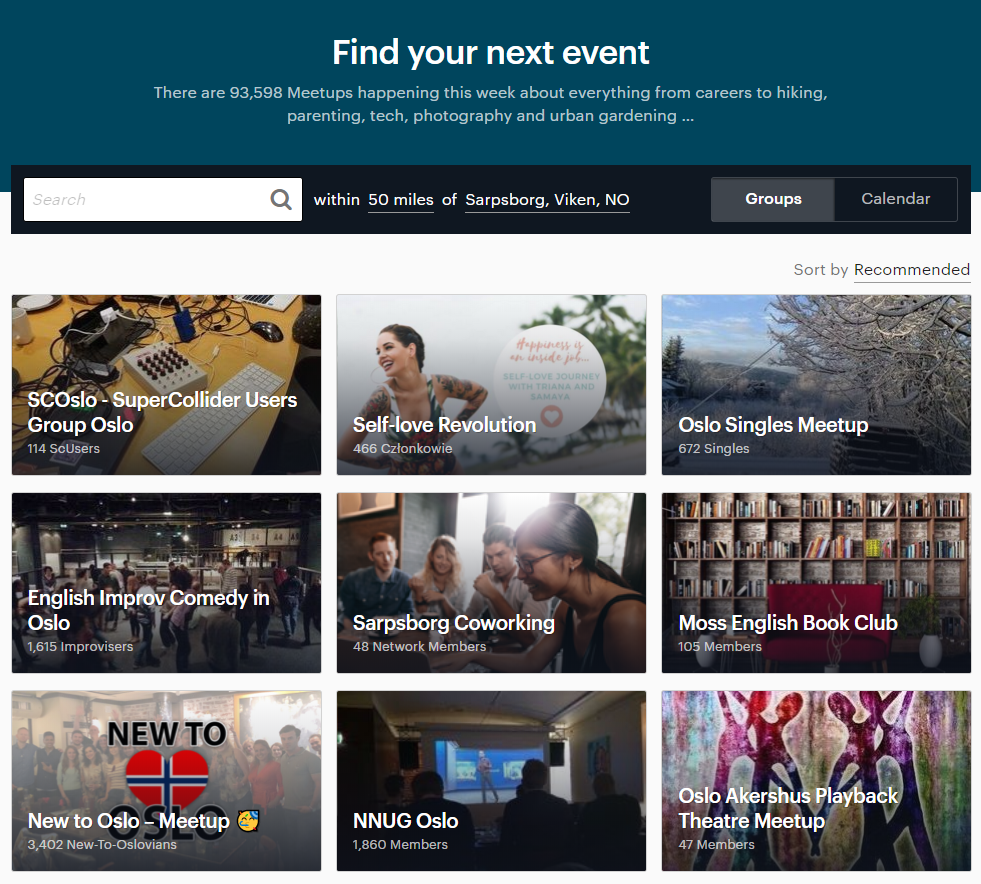
\includegraphics[width=0.48\textwidth]{Illustrasjoner/andre_platformer/meetup_forside.png}
  \end{center}
  \caption{Forsidevisning på Meetup.com etter innlogging.}
\end{wrapfigure}
%END FIGURE%

Etter tvungen brukerregistrering på Meetup.com blir man presentert en forside med en rekke kort som representerer relevante aktiviteter for bruker i geografisk område. 

\vspace{5mm} %5mm vertical space

Ved klikk på et av arrangementene møtes man med en informasjonsside som blant annet informerer om lokasjon, antall medlemmer, organisator, kommende datoer m.m.

\vspace{5mm} %5mm vertical space

I navigasjonen har bruker tilgang på en utforsk-knapp som går til en søkeside, meldinger fra andre brukere og notifikasjoner om relaterte hendelser.

\vspace{5mm} %5mm vertical space

Prosjektgruppen opplever Meetup.com som en nokså ryddig side, dog med minimal aktivitet i Norge. Det er ingen savn etter ytterligere informasjon fra de ulike arrangementene, og det bør bli vurdert lignende implementasjon ved organisasjonssidene som skal utformes på Aktiv Student.

\newpage

NyBy er et verktøy for kommuner og organisasjoner ment for å løse viktige velferdsoppgaver i samarbeid med ansatte og innbyggere\footnote{https://nyby.no/hva-er-nyby}. Kommuner legger ut en henvendelse via meldinger på en app, som medlemmer av frivillige organisasjoner i nærheten kan velge å svare på. Målet er mer direkte kommunikasjon mellom behov og støtte, som igjen vil føre til spart tid og kommunale ressurser.

\vspace{5mm} %5mm vertical space

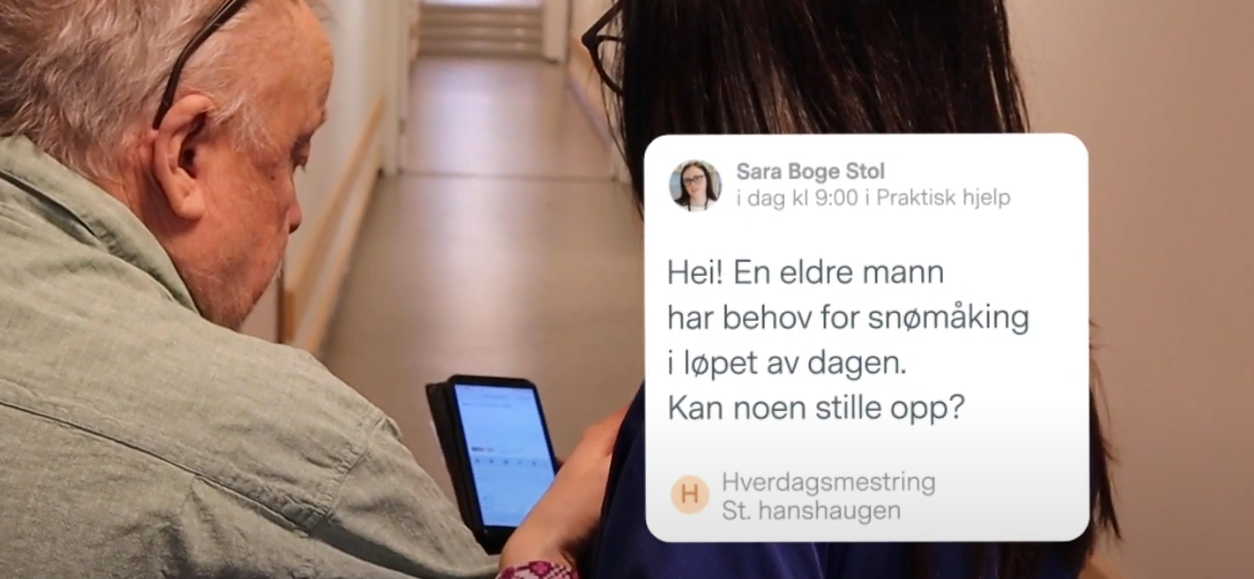
\includegraphics[width=\textwidth]{Illustrasjoner/andre_platformer/nyby_henvendelse.png}

\vspace{5mm} %5mm vertical space
%BEGIN FIGURE%
\begin{wrapfigure}{r}{0.5\textwidth}
  \begin{center}
    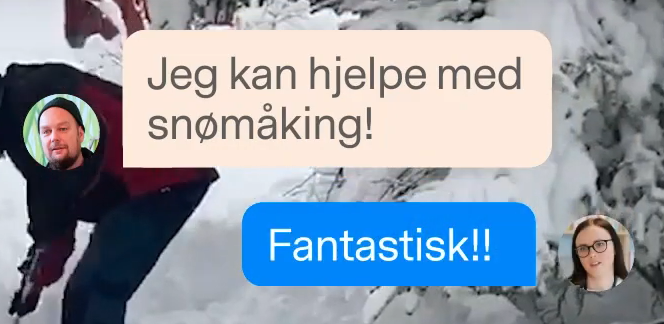
\includegraphics[width=0.48\textwidth]{Illustrasjoner/andre_platformer/nyby_svar.png}
  \end{center}
  \caption{Skjermdump informasjonsvideo fra nyby.no}
\end{wrapfigure}
%END FIGURE%
Via en app kan de som har behov for hjelp melde seg inn i lokale grupper og spørre om bistand til å gjøre mindre ærender. I samme appen kan de som har mulighet til å hjelpe til respondere til den som trenger hjelp.

\vspace{5mm} %5mm vertical space

Prosjektgruppen er imponert over effektiviteten over denne type kommunikasjon ved behov for hjelp. Mange mennesker kan få hjelp til ting som for noen er enkle, men for andre særskilt vanskelig. Dette ved å kutte ut flere ledd innenfor kommunale sektorer, hvor ressursene kan brukes på noe annet. Covid-19 og dens medfølgende karantenetiltak setter desto større fokus på denne type bidrag til samfunnet.

\vspace{5mm} %5mm vertical space

Nextdoor.com setter søkelys på forholdet mellom naboer\footnote{https://global.nextdoor.com/}. Ved registrering kreves verifisering av bostedsadresse, noe som sørger for at brukere kun kan forholde seg til de som bor nær hverandre. Norge er per dags dato ikke et av landene som støttes av Nextdoor, men nettsiden opplyser om et ønske å spre seg til alle land.

\vspace{5mm} %5mm vertical space

Gruppen ser et sterkt fokus på geografisk lokasjon. Selv over nettet så kan miljøet rundt brukere oppfattes veldig personlig, da tjenesten komprimeres kun til de respektive nabolagene.

\vspace{5mm} %5mm vertical space

MeetMe\footnote{https://www.meetme.com/home} og Skout\footnote{https://www.skout.com/} kan sees på som varianter av Tinder, applikasjoner for mennesker i samme geografisk nærområde, som blir definert gjennom fellestrekk i brukerprofilene.

\vspace{5mm} %5mm vertical space

Noe alle evaluerte nettsider har til felles, er at de krever registrering og innlogging. Det foreligger som en naturlig funksjon, da de fleste gjøremål trenger identifisering av bruker. Aktiv Student sitt utgangspunkt er brreg.no, en oversikt over ulike fritidsorganisasjoner, lag og foreninger i Norge. Ved å sammenligne den type innhold med andre oversikter som finnes (finn.no, ut.no, gulesider.no etc), så krever fåtallet av de innlogging. Det forblir da et mål fra prosjektgruppens sin side om å prøve å utelate innlogging, ihvertfall forenkle prosessen betraktelig. Prosjektgruppen diskuterte de forskjellige tjenestene på grunnlag av interessante funksjoner, men også på basis av Jakob Nielsens 10 prinsipper for design av brukergrensesnitt\footnote{https://www.nngroup.com/articles/ten-usability-heuristics/}.

% --------------------- Dette må fullføres ----------------------------- %
\subsection{Relaterte studier og publikasjoner}
De fleste aspektene med oppdraget er forsket på og skrevet om i studier og publikasjoner. Utvikling av søkemotorer og oppslagsverk er gjort før og det finnes nok av dokumentasjon av dette. Prosjektgruppen valgte derfor å trekke fram de mest sentrale aspektene som, når satt sammen, skilte tjenesten beskrevet i oppdraget fra andre tjenester og bidro til at den kunne dekke et behov i markedet. Aspektene som ble trukket fram var {\em gjøre det enklere å delta}, {\em oppfordre til deltakelse sammen med andre}, {\em interaksjon med andre brukere} og {\em foreslå aktiviteter for brukerne}. Disse ble undersøkt nærmere ved hjelp av relaterte studier og publikasjoner.

\paragraph{Gjøre det enklere å delta}
Målet med oppdraget var å lage en tjeneste som gjorde det enklere å finne organisasjoner, lag og foreninger, men for å få noe ut av tjenesten ville det også være helt sentralt å legge opp til at det skulle være enkelt å ta steget for å faktisk delta på aktiviteter. 

Forskningsartikkelen {\em To Go or not to Go!: What Influences Newcomers of Hybrid Communities to Participate Offline} \cite{NEWCOMERS:4:CT17} tar utgangspunkt i tjenesten Meetup, beskrevet i delkapittel~\ref{section:relaterte-tjenester} og~\ref{section:benchmarking}, og undersøkte hvilke faktorer som kunne spille inn for at brukere skulle ta steget til å møte opp på en aktivitet for første gang. Funn fra artikkelen pekte mot flere faktorer som kunne øke sjansen for deltakelse, blant annet {\em utfyllende beskrivelse av arrangementet og instruksjoner for deltakelse
}, {\em at mange andre skulle delta}, {\em inkluderende og velkommende ordbruk i beskrivelsen} og {\em kort sosial distanse mellom bruker og arrangør, slik at det ikke ble truende å ta kontakt}. 

Andre aspekter som kunne vært relevant men som ikke var nevnt i artikkelen var blant annet {\em om vanskeligheter med å finne fram til interessante aktiviteter eller riktig informasjon kunne være en hindring for deltakelse} og om {\em muligheten for å kommunisere med andre potensielle deltakere i et digitalt sosialt felleskap kunne øke sjansen for deltakelse}.

\paragraph{Oppfordre til deltakelse sammen med andre}
Notater:
Det har blitt skrevet om digitale tjenester som oppfordrer brukere til å delta på gruppeaktiviteter i {\em Group-Activity Organizing Through an Awareness-of-Others Interface} \cite{AWARENESS:3:CSCW18}. Artikkelen tar utgangspunkt i en app som lar brukere organisere aktiviteter og andre brukere delta på disse. Fokuset ligger på å gjøre organiseringen og gjennomføringen av aktiviteter så lett som mulig.

\paragraph{Interaksjon med andre brukere}
Notater:
Det er også skrevet artikler om å få ukjente til å ta kontakt med hverandre på digitale tjenester. {\em Outlining the design space of playful interactions between nearby strangers} \cite{NEARBY:5:AM16} beskriver en designprosess med workshops for å utvikle ideer for hvordan fremmede mennesker som befinner seg i nærheten av hverandre kan samhandle på forskjellige måter. {\em Playfulness and progression in technology-enhanced social experiences between nearby strangers} \cite{PLAYFUL:6:NORDICHI18} beskriver videreføringen av denne prosessen, der en app som heter Next2You blir utviklet etter prinsippene fra design-workshops og testet i et bruker-studie. Appen lar brukerne automatisk utveksle valgfri informasjon med andre brukere som kommer innen mobiltelefonens Bluetooth-radius.

\paragraph{Foreslå aktiviteter for brukere}
Notater:
Anbefaling av aktiviteter har blitt skrevet om i artiklene {\em A Novel Method for Event Recommendation in Meetup} \cite{MEETUP:7:ASONAM17} og {\em Users psychological profiles for leisure activity recommendation: user study} \cite{PROFILES:10:CITREC17}. Begge disse artiklene samler inn store mengder informasjon om brukere som brukes til å beregne hvilke aktiviteter som kan være interessante og foreslå disse for brukeren.

\paragraph{Fritid med bistand}
Notater:
Publikasjonene {\em Fritidsorganisasjoner vil og de kan} \cite{FRITID:12}, {\em Inkludering gjennom organiserte fritidsaktiviteter} \cite{INKLUDERING:11} og {\em Tillit, mestring og selvoppfatning} \cite{TILLIT:13} har fokus på aktivisering hos personer med nedsatt funksjonsevne, lav inntekt eller andre tydelige hindringer som gjør at de kan trenge støtte for å delta på aktiviteter. Disse publikasjonene er relatert til Anders Midtsundstad sin metode {\em Fritid med Bistand} \footnote{https://www.fritidmedbistand.no/}. 
% ---------- Annen tittel enn Nye aspekter etc?---------------%
\paragraph{Nye aspekter jobbet med i prosjektoppgaven}
Notater:
Mange av ideéne og prinsippene som er beskrevet i disse artiklene tas med videre av prosjektgruppen i arbeidet med tjenesten. Det er flere aspekter av dette bachelorprosjektet som ikke er beskrevet i publikasjonene nevnt ovenfor. En av disse er autonomi hos brukeren. Et viktig poeng med oppdraget er at brukeren selv skal ville dele informasjon, ta kontakt og delta på aktiviteter. Det vil både være best for brukeren og enklest for utviklingsteamet om brukeren selv velger hvilken informasjon som skal deles. Et annet aspekt som er lite sett på er involveringen av allerede eksisterende organisasjoner og hvordan brukerens deltakelse kan berike både organisasjonene og nærmiljøet sitt. 

I tillegg er det slik at de fleste studiene fokuserer enten på brukere som allerede er sosiale og ikke har problemer med å ta kontakt med andre, eller brukere som har ulike hindringer eller funksjonsnedsettelser som øker terskelen for at de vil ta kontakt eller delta. Ved at målgruppen i dette oppdraget er først og fremst alle studenter ved HIØ vil tjenesten i dette bachelorprosjektet ta hensyn til alle typer mennesker med forskjellige grader av sosiale preferanser, forskjellige motivasjoner, og også personer med forskjellige typer nedsatt funksjonsevne.

\section{Rapportstruktur}
\paragraph{Kapittel 2} inneholder en beskrivelse av arbeidsprosessen med billedlig og skriftlig dokumentasjon, brukerundersøkelser, utvikling av skisser, brukertesting, evalueringer og forbedringer som er gjort.

\paragraph{Kapittel 3}
inneholder en beskrivelse av det det ferdige resultatet som gruppen produserte og en evaluering av dette fra studenter, organisasjoner, fagpersoner og oppdragsgiver.

\paragraph{Kapittel 4}
diskuterer resultatet og om det oppnådde krav og spesifikasjoner satt på forhånd. Her vil det foreligge en vurdering av prosjektet og arbeidet fra prosjektgruppen og anbefalinger og designprinsipper for videre arbeid. Gruppen vil også diskutere erfaringer gjort underveis i arbeidet. Avslutningsvis legges det frem en konklusjon og oppsummering.

